\section{Physics Informed Neural Networks (PINNs)}
\label{sec:pinn}
\subsection{Deep Feedforward Neural Network}

Deep feedforward neural network, also known as a multilayer perceptron (MLP), is a simple structure of function approximator commonly used in machine learning. It maps a given input $\mathbf{x}$ to an output through successive affine-linear mappings and non-linear transformations, which can be described in a composite function for $K$-layer neural network such that:
\begin{equation}
    \label{eqn:k_layer_nn}
    \mathcal{N_{\mathbf{\boldsymbol\theta}}}(\mathbf{x})=L_K\circ\sigma\circ L_{K-1}\dots\circ\sigma\circ L_1,
\end{equation}
where $\circ$ denotes function composition; $L$ is an affine mapping and is given more explicitly $L_k\mathbf{x}_k=\mathbf{W}_k\mathbf{x}_k+\mathbf{b}_k$ in which $\mathbf{W}_k \in \mathbb{R}^{n_{k+1}\times n_{k}}$ are the weights of the network, $\mathbf{b}_k \in \mathbb{R}^{n_{k+1}}$ represents the bias vector, $\mathbf{x}_k \in \mathbb{R}^{n_{k}}$ is an input vector for $k$ representing the $k$-th hidden layer including $n_k$ neurons; $\sigma$ is a nonlinear activation function, and $\mathbf{\boldsymbol\theta}=\big\{\mathbf{W}_k,\mathbf{b}_k  \big\}_{1 \le k \le K}$. An illustration of a deep feedforward neural network is given in \figref{fig:pinn}. 

\subsection{PINNs as a PDE Solver and Parameter Estimator}

Let $\Omega \subset \mathbb{R}^{n}$ be the domain of interest with a boundary defined as $\partial \Omega$ for some $n \geq 1$. An abstract representation of a PDE and relevant boundary conditions can be written as:
\begin{equation}
\label{eqn:abstract_pde}
\begin{split}
     \mathcal{D}(\xi(\mathbf{x}))=0 \quad \mathbf{x} \in \Omega, \\ \mathcal{B}(\xi,\mathbf{x})=0 \quad on \,\, \partial \Omega,
\end{split}
\end{equation}
where $\mathcal{D}$ is a spatial-temporal differential operator operating on the PDE solution $\xi$; $\mathcal{B}(\xi,\mathbf{x})$ can be any type of boundary conditions (Dirichlet, Neumann, Robin or mixed). Moreover, we assume that $\mathbf{x}$ includes a temporal parameter $t$ for time-dependent PDEs.

PINNs solve a PDE by satisfying the physics and boundary conditions subject to a neural network $\mathcal{N_{\mathbf{\boldsymbol\theta}}}(\mathbf{x})$ that approximates to the solution of a PDE $\xi(\mathbf{x})$. Any derivatives of the network outputs $\tilde{\xi}(\mathbf{x})$ with respect to the inputs defining a PDE as well as needed derivatives for boundary conditions are computed via automatic differentiation (AD)~\cite{bprs:18}, which applies the chain rule to compute the derivatives of a compositional function. If we define the training data for a PDE as $\Omega_p \subset \Omega$ and for boundary conditions as $\partial \Omega_b \subset \partial \Omega $, the total loss function can be written such that:
\begin{equation}
    \label{eqn:loss_function}
    \mathcal{L}(\boldsymbol\theta) = w_p \frac{1}{|\Omega_p|}\sum_{\mathbf{x} \in \Omega_p} ||\mathcal{D}(\tilde{\xi}(\mathbf{x}))||+w_b \frac{1}{|\partial \Omega_b|}\sum_{\mathbf{x} \in \partial \Omega_b} ||\mathcal{B}(\tilde{\xi},\mathbf{x})||.
\end{equation}
Here, the $L_2$ norm $||\cdot||$ is applied to the PDE residual in the first term, and to the boundary conditions in the second term of the loss function.

The objective is to find an optimal $\boldsymbol\theta$ which minimizes the loss function $\mathcal{L}(\boldsymbol\theta)$ by a chosen gradient based optimizer. The illustration of a PINN procedure is given in \figref{fig:pinn}. 

\begin{figure}
 \centering
 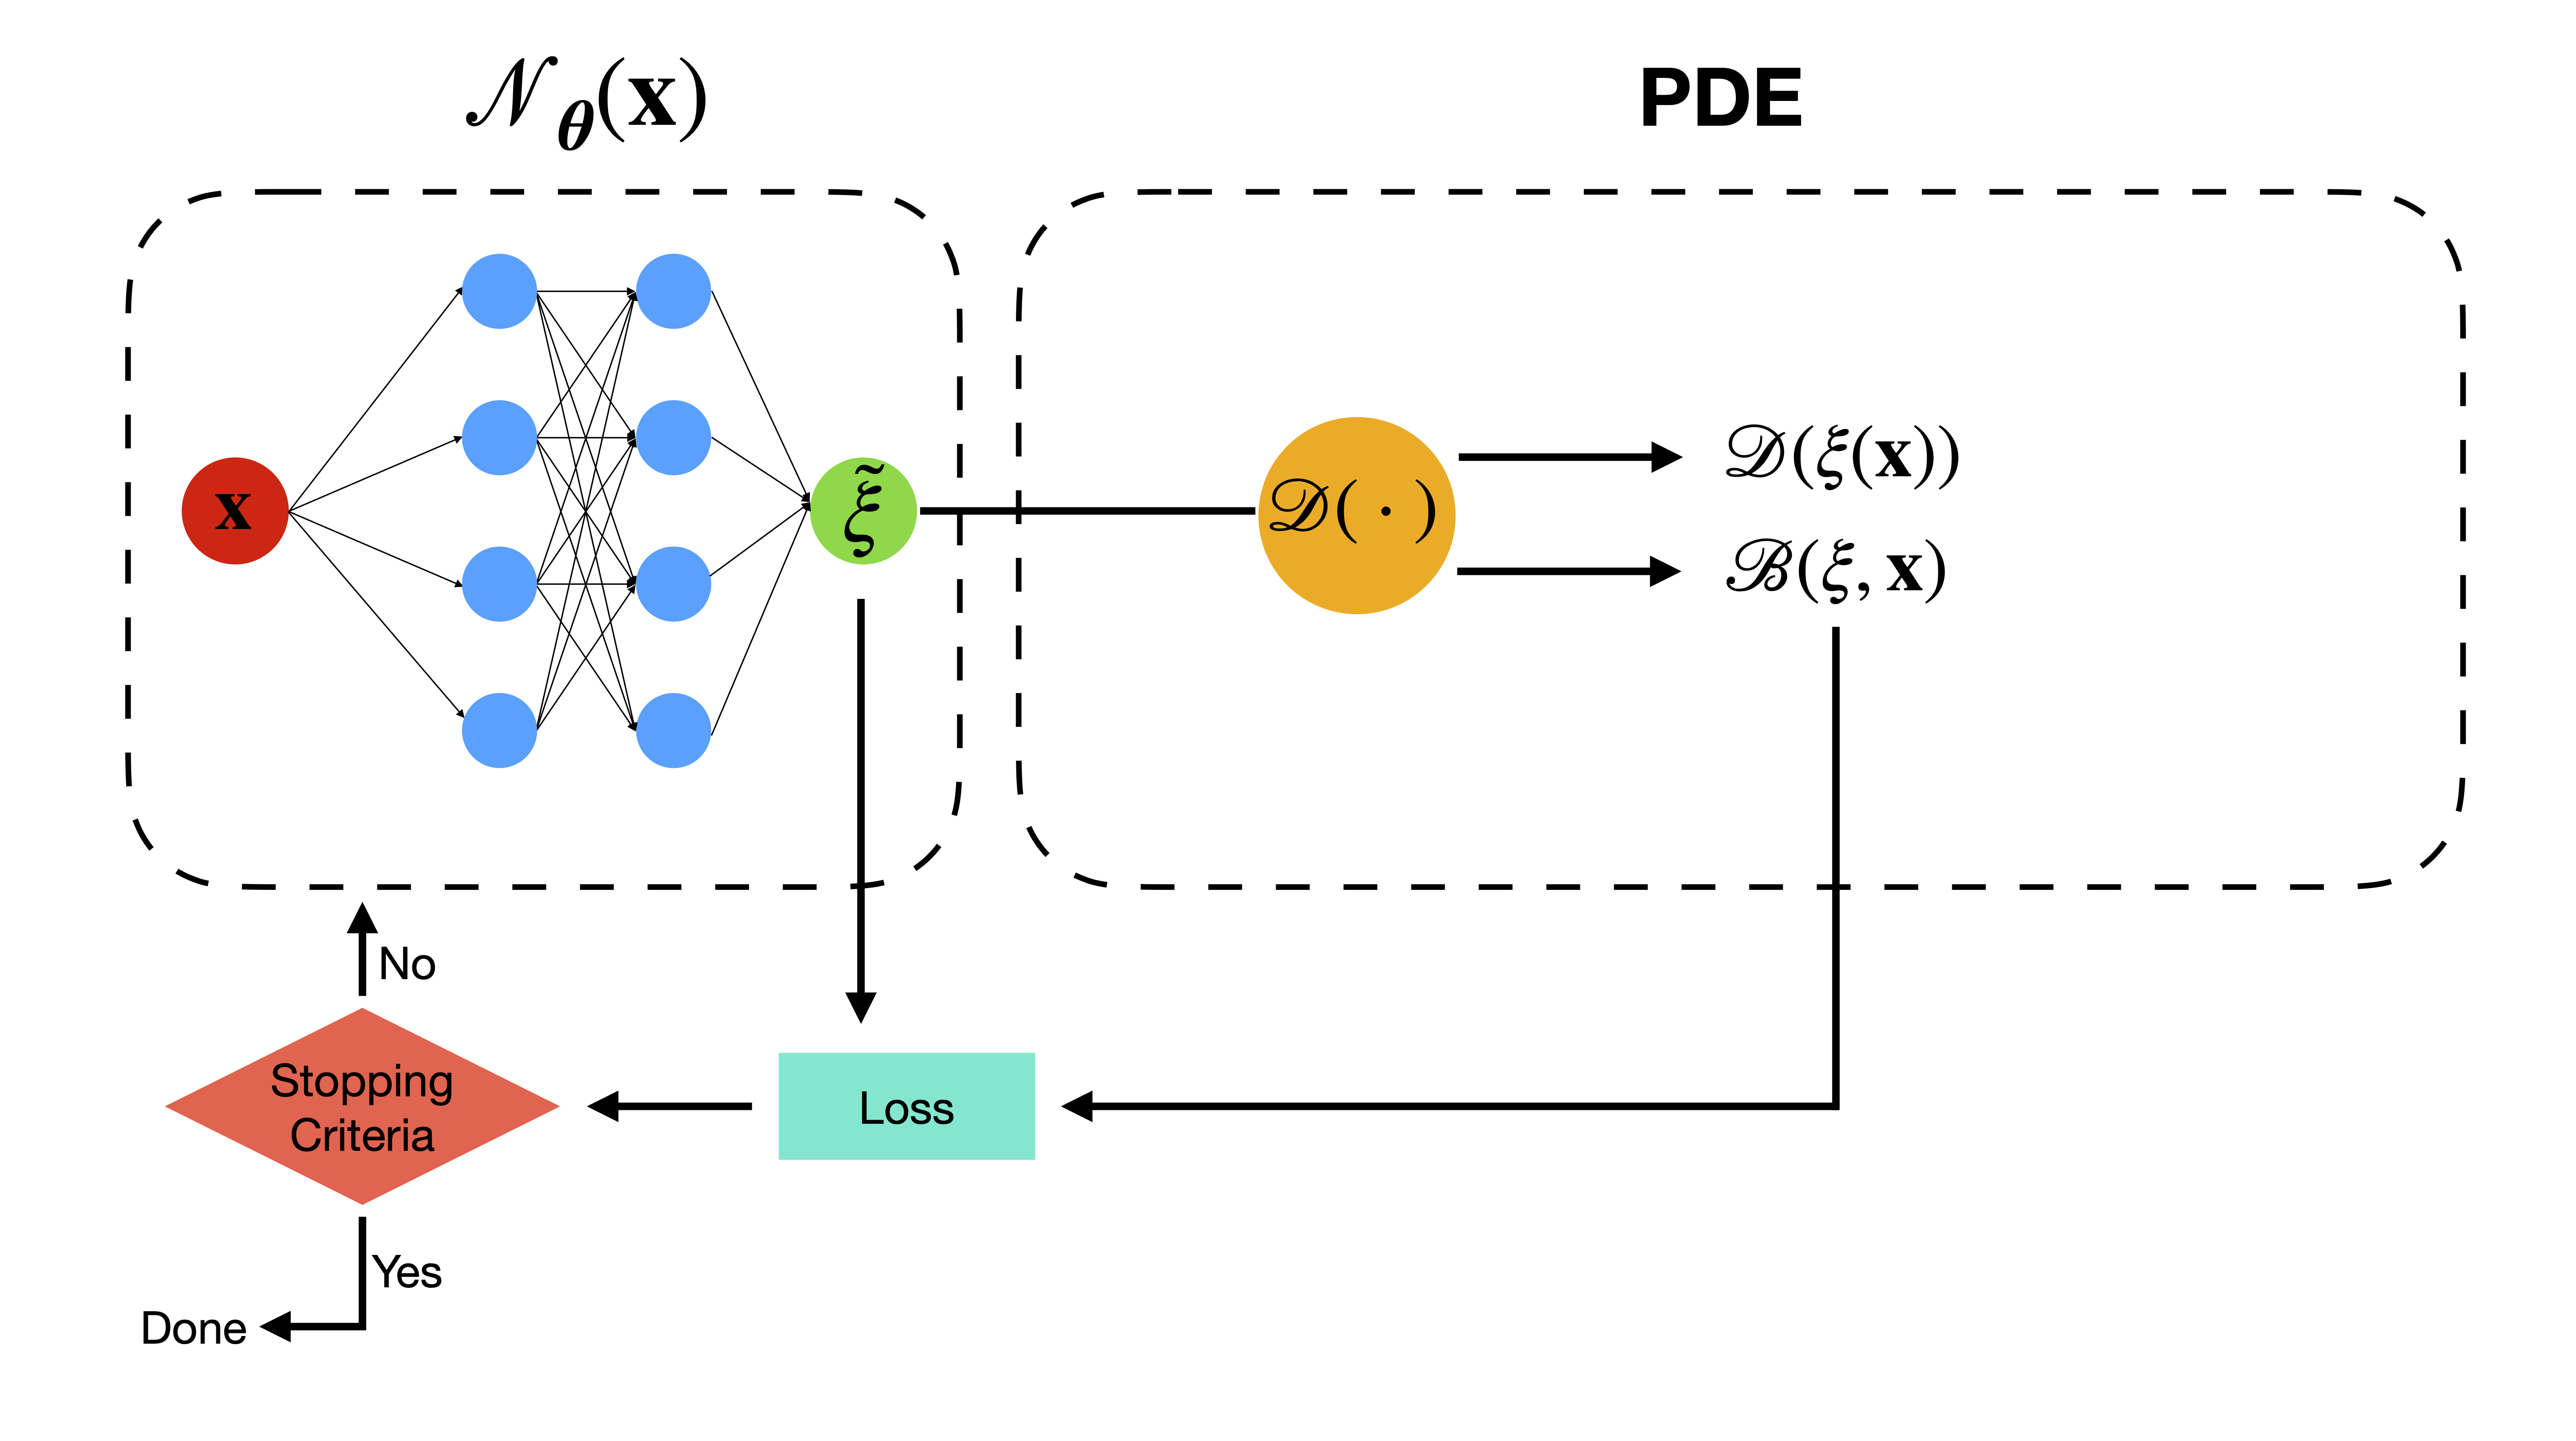
\includegraphics[width=0.9\textwidth]{figures/chap02_preliminaries/pinn.png} 
 \caption{An illustration of a physics informed neural network procedure.}
 \label{fig:pinn}
\end{figure}

Considering an inverse problem, let's rewrite the definition of an abstract PDE \eqref{eqn:abstract_pde} parameterized by $\boldsymbol\gamma$ such that:
\begin{equation}
    \label{eqn:gamma_pde}
    \mathcal{D}(\xi(\mathbf{x});\boldsymbol\gamma)=0 \quad \mathbf{x} \in \Omega.
\end{equation}
Moreover, let's assume we know the solution $\xi(\mathbf{x})$ on some points $\Omega_d \subset \Omega$. In this case, the unknown parameter $\boldsymbol \gamma$ can also be predicted by PINNs just by adding an extra loss term to the loss we defined earlier in a way that 
\begin{equation}
\label{eqn:total_loss}
\begin{split}
       \mathcal{L}(\boldsymbol\theta, \boldsymbol \gamma) &= w_p \frac{1}{|\Omega_p|}\sum_{\mathbf{x} \in \Omega_p} ||\mathcal{D}(\tilde{\xi}(\mathbf{x}); \boldsymbol \gamma)||\\&\quad +w_b \frac{1}{|\partial \Omega_b|}\sum_{\mathbf{x} \in \partial \Omega_b} ||\mathcal{B}(\tilde{\xi},\mathbf{x})||\\&\quad   + w_d \frac{1}{|\Omega_d|}\sum_{\mathbf{x} \in \Omega_d} ||\tilde{\xi}(\mathbf{x})-\xi(x)||,
\end{split}
\end{equation}
where $w_p$, $w_b$, and $w_d$ are the weights of the PDE residual term, boundary term, and data fitting term, respectively. Then, the optimization goal becomes
\begin{equation}
    \label{eqn:optimization}
    \text{finding} \,\, \boldsymbol\theta \,\, and \,\, \boldsymbol\gamma \,\, :     \underset{\boldsymbol\theta,\boldsymbol\gamma}{\arg\min}\,\, \mathcal{L}(\boldsymbol\theta,\boldsymbol\gamma). 
\end{equation}